\documentclass[a4paper]{jarticle}

\usepackage{moreverb}
\usepackage{ascmac}
\usepackage{amsmath}
\usepackage{enumerate}
\usepackage{eclbkbox}
\usepackage[dvipdfmx]{graphicx}

\setlength{\textheight}{\paperheight}   % 紙面縦幅を本文領域にする(BOTTOM=-TOP)
\setlength{\topmargin}{4.6truemm}       % 上の余白を30mm(=1inch+4.6mm)に
\addtolength{\topmargin}{-\headheight}  % 
\addtolength{\topmargin}{-\headsep}     % ヘッダの分だけ本文領域を移動させる
\addtolength{\textheight}{-60truemm}    % 下の余白も30mm(BOTTOM=-TOPだから+TOP+30mm)

\setlength{\textwidth}{\paperwidth}     % 紙面横幅を本文領域にする(RIGHT=-LEFT)
\setlength{\oddsidemargin}{-0.4truemm}  % 左の余白を25mm(=1inch-0.4mm)に
\setlength{\evensidemargin}{-0.4truemm} % 
\addtolength{\textwidth}{-50truemm}     % 右の余白も25mm(RIGHT=-LEFT)

\begin{document}
\title{センシング工学特論\\レポート課題【課題 I 】}
\author{3G150131 松井 健人}
\date{2015年6月5日}
\maketitle

%-----------------------------
%1章
%-----------------------------

\section{課題 I }
\textbf{観測方程式}
\begin{equation}
z = x_0 + {x_1}a + {x_2}{a^2} = 
\left[  \ 1\ \ a\ \ a^2\   \right]
 \begin{bmatrix}
{x_0} \\ {x_1} \\{x_2} \\ 
\end{bmatrix}   + w= 
\mbox{\boldmath $a$}^{T}\mbox{\boldmath $x$} + w
\end{equation}
に関して下表の観測値が得られた.

\begin{table}[hbtp]
 \caption{C言語の代表的なデータの型}
 \label{table:data_type}
 \begin{center}
  \begin{tabular}{rc|rc|rc|rc}
   \hline
   a & z & a & z & a & z& a & z \\
   \hline \hline
   -15 & 162.1746 & -8& 26.5951 & 0 & -1.9845  & 8 & 93.7607\\
   -14 & 139.5805 & -7 & 20.1832 & 1 & 2.0593  & 9 & 112.6638\\
   -13 & 113.8133 & -6 &  8.8816 & 2 & 12.3849  & 10 & 134.9818 \\
   -12 & 94.3372  & -5 &   1.8636 & 3 & 17.9044  & 11 &162.7143\\
   -11 & 74.7258  & -4 &  -5.0213& 4 & 30.1826  & 12 &188.9610 \\
   -10 & 59.3817  & -3 & -5.8861 & 5 & 41.1677  & 13 &219.6236 \\
   -9  & 41.4117   & -2 &   -5.7711& 6 & 55.7128 & 14 & 248.9036 \\
        &               & -1 &   -4.9332& 7&  74.2944  & 15 & 281.3082\\
   \hline
  \end{tabular}
 \end{center}
\end{table}

なお,$a$が奇数のときの観測雑音$w$は平均値0,分散1の正規分布であり,$a$が偶数のときの観測雑音の$w$は平均値0,分散4の正規分布である. 

\begin{enumerate}[(1)]
\item バッチ型最小二乗法,逐次型最小二乗法それぞれにより未知数(一定値)$x$を推定するアルゴリズムを示せ.
また,実際にプログラムを作成して推定値を求めよ.プログラミング言語としては何を用いてもよいが最小二乗法の関数は使わないこと.

\item 逐次型最小二乗法において,推定値の初期共分散に対する推定精度への影響を調べよ.
\end{enumerate}

ただし,$x$の解は\(
\begin{bmatrix}
{x_0} \\ {x_1} \\{x_2} \\ 
\end{bmatrix} =
\begin{bmatrix}
{-3} \\ {4} \\{1} \\ 
\end{bmatrix}
\)
である.

%-----------------------------
%2章
%-----------------------------
\newpage
\section{最小二乗法による未知数の推定}
\subsection{最小二乗法}
最小二乗法とは,観測により得た数値を1次関数や対数曲線などの関数を用いて近似する際に,誤差の二乗和が最小となる係数を決定することで未知数を推定する手法である.
未知数の推定方法は大きく分けて、先験情報と観測値から推定するベイズ推定と観測値のみにより推定するフィッシャー推定の2つに分類され,最小二乗法はフィッシャー推定に分類される.
また,最小二乗法にはバッチ型最小二乗法と逐次型最小二乗法がある.


\subsection{バッチ型最小二乗法}
\subsubsection{バッチ型最小二乗法による推定アルゴリズム}
バッチ型最小二乗法とは,任意の時刻における未知数を推定するために,それ以前に観測された数値を一括で処理する方法である.この方法では,多くのデータを扱うこととなるため,計算時間が増大し,大きなメモリ容量が必要となる.

バッチ型最小二乗法では,複数の観測値を扱うので観測方程式(1)を式(2)のように変換する.
\begin{equation}
\begin{bmatrix}
{z_{(1)}} \\ \vdots \\{z_{(k)}} \\ 
\end{bmatrix} =  
\begin{bmatrix}
{\mbox{\boldmath {$H$}}_{(1)}} \\ \vdots \\{\mbox{\boldmath {$H$}}_{(k)}} \\ 
\end{bmatrix}
\mbox{\boldmath $x$} +
\begin{bmatrix}
{w_{(1)}} \\ \vdots \\{w_{(k)}} \\ 
\end{bmatrix}
\iff
\mbox{\boldmath $z$}^k
=
\mbox{\boldmath $H$}^k
\mbox{\boldmath $x$}
+
\mbox{\boldmath $w$}^k
\end{equation}

また,観測雑音${\mbox{\boldmath $w$}^k}$の共分散${\mbox{\boldmath $R$}^k}$を式(3)に示す.

\begin{flalign}
\mbox{\boldmath $R$}^k =
\begin{bmatrix}
{\mbox{\boldmath $R$}_{(1)}} & \cdots & 0\\
 \vdots & \ddots & \vdots\\
0 & \cdots & {\mbox{\boldmath $R$}_{(k)}} \\ 
\end{bmatrix} 
\vspace{3mm}
\end{flalign}

推定値および推定誤差共分散は式(2), (3)よりそれぞれ式(4)および(5)と表すことができる.

\begin{equation}
\mbox{\boldmath $\hat{x}$}_{(k)} =
\left[ 
(\mbox{\boldmath $H$}^k)^{T}
(\mbox{\boldmath $R$}^k)^{-1}
\mbox{\boldmath $H$}^{T}
\right]^{-1}
(\mbox{\boldmath $H$}^k)^{T}
(\mbox{\boldmath $R$}^k)^{-1}
\mbox{\boldmath $z$}^k
\vspace{3mm}
\end{equation}
\begin{equation}
\mbox{\boldmath $P$}_{(k)} =
\left[ 
(\mbox{\boldmath $H$}^k)^{T}
(\mbox{\boldmath $R$}^k)^{-1}
\mbox{\boldmath $H$}^{T}
\right]^{-1}
\vspace{3mm}
\end{equation}

バッチ型最小二乗法では未知数を式(4)を用いて推定する.


\newpage
\subsubsection{バッチ型最小二乗法により推定するプログラム}
バッチ型最小二乗法により未知数を推定するプログラムをオブジェクト指向スクリプト言語Rubyで作成した.今回は時刻$a$が-15から15までを想定して各時刻における未知数の推定を行うが,項が3つ存在するので過去の観測データが3つ必要なる.そのため,時刻$a$が-13となってから推定を開始する.
ソースコードをリスト 1に示す.
また,出力結果をリスト 2に示し,推定値の時系列グラフを図 1に示す.
時刻$a$が-13,-12のとき推定値の誤差が大きいため,それらの時刻を除いた推定値の時系列グラフを図 2に示す.

\vspace{3mm}
\begin{center}
リスト 1: バッチ型最小二乗法により推定するプログラムのソースコード
\begin{small}
\vspace{1mm}
\listinginput{1}{sencing1-2_20150605.rb}
\end{small}
\vspace{3mm}
\end{center}

\begin{center}
リスト 2: バッチ型最小二乗法により推定するプログラムの出力結果
\begin{small}
\vspace{1mm}
\listinginput{1}{BatchDatasHIDE.txt}
\end{small}
\end{center}
\clearpage
\begin{figure}[!h]
  \centering
  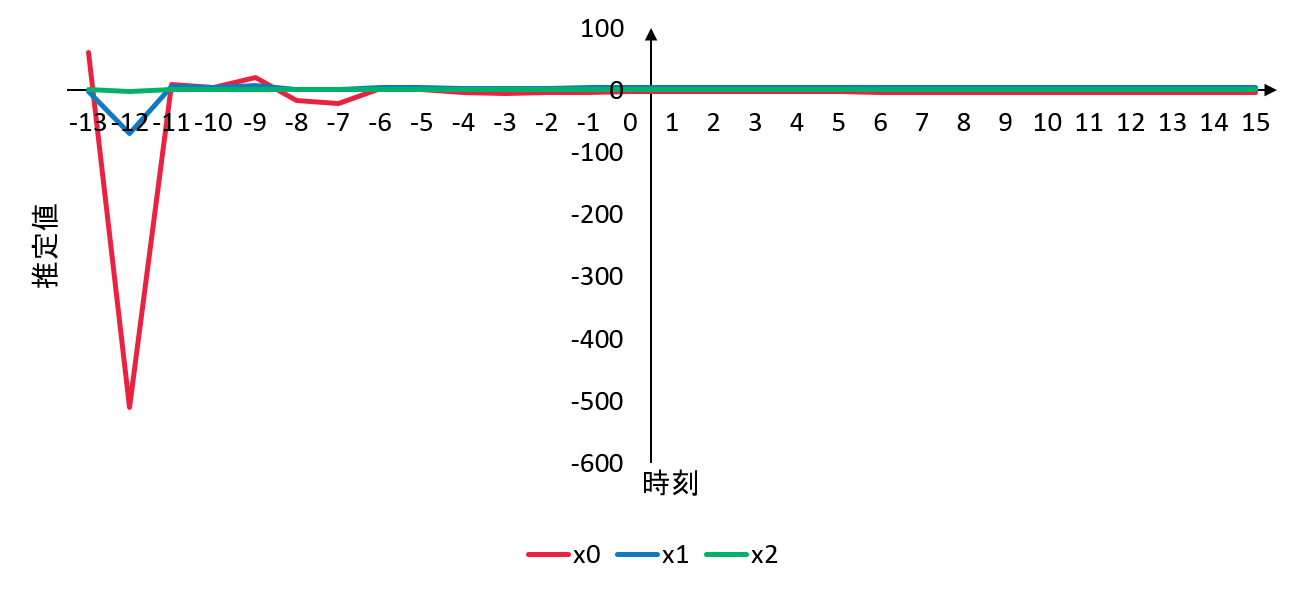
\includegraphics[width=16cm]{batch1.png}
  \caption{バッチ型最小二乗法による推定値の時系列グラフ(-13$\le a \le $15)}
 \label{graph}
\end{figure}

\begin{figure}[!h]
  \centering
  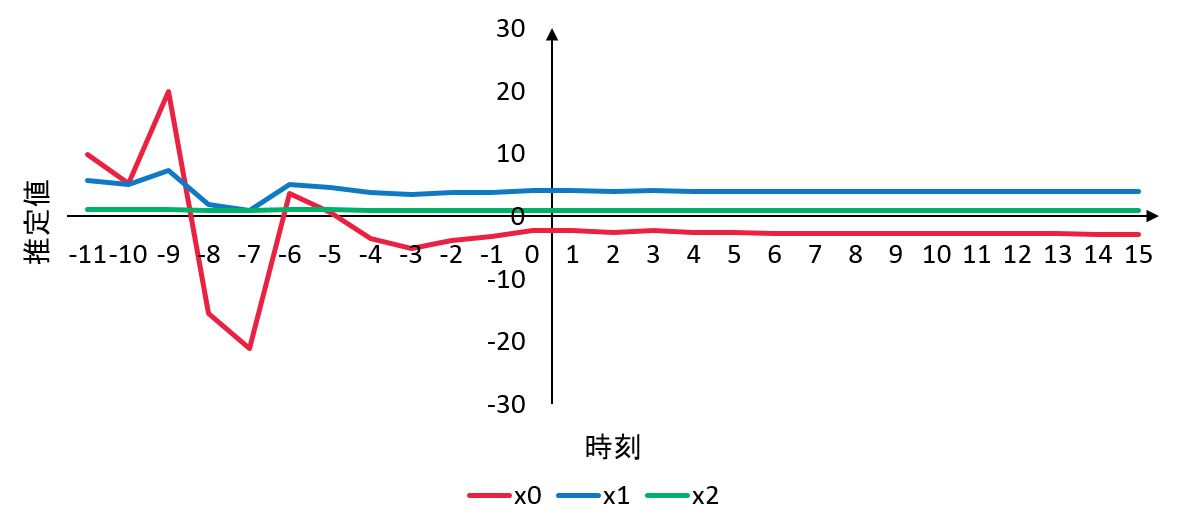
\includegraphics[width=16cm]{batch2.png}
  \caption{バッチ型最小二乗法による推定値の時系列グラフ(-11$\le a \le $15)}
 \label{graph}
\end{figure}

リスト2より,時刻$a$が15のとき推定値は\(x_{0}=-2.833, x_1 = 3.991 x_2 = 1.001\) となっており,正しく推定できていることがわかる.また,図1,2より,推定値が収束していることがわかる.
%-----------------------------
%2.3章
%-----------------------------

\clearpage
\subsection{逐次型最小二乗法}\label{program}
\subsubsection{逐次型最小二乗法による推定アルゴリズム}
逐次型最小二乗法とは,任意の時刻における未知数を推定するために,その時刻の1つ前の時刻において推定した数値を補正する方法である.
この方法では,任意の時刻の1つ前の時刻の推定値が必要となるが,最初の時刻では,1つ前に推定値が存在しないため推定することができない.
そこで,最初の数サイクルにおいてバッチ型最小二乗法を用いて推定値および推定誤差共分散を導出する,あるいは,推定値を0とし,推定誤差共分散を非常に大きい値とする必要がある.ここで,推定誤差共分散が非常に大きい場合,その推定値は信用出来ないことを意味する.

バッチ型最小二乗法では,複数の観測値を扱うので観測方程式(1)および観測雑音の共分散,推定誤差共分散により観測予測誤差共分散を求める.
推定誤差共分散からフィルタゲインを求める.
観測予測誤差共分散およびフィルタゲインを式(6), (7)に示す.

\begin{equation}
\mbox{\boldmath ${S}$}_{(k+1)} =
\mbox{\boldmath $H$}_{(k+1)} 
\mbox{\boldmath $P$}_{(k)} 
{\mbox{\boldmath $H$}^{T}}_{(k+1)}
+
\mbox{\boldmath $R$}_{k+1}
\vspace{3mm}
\end{equation}
\begin{equation}
\mbox{\boldmath ${W}$}_{(k+1)} =
\mbox{\boldmath $P$}_{(k)} 
{\mbox{\boldmath $H$}^{T}}_{(k+1)}
{\mbox{\boldmath $S$}^{-1}}_{(k+1)}
\vspace{3mm}
\end{equation}

推定値および推定誤差共分散は式(6), (7)よりそれぞれ式(8)および(9)と表すことができる.

\begin{equation}
\mbox{\boldmath $\hat{x}$}_{(k+1)} =
\mbox{\boldmath $\hat{x}$}_{(k)}+
\mbox{\boldmath ${W}$}_{(k+1)}
\left[ 
z_{(k+1)}-
\mbox{\boldmath $H$}_{(k+1)} 
\mbox{\boldmath $\hat{x}$}_{(k)}
\right]
\vspace{3mm}
\end{equation}
\begin{equation}
\mbox{\boldmath $P$}_{(k+1)} =
\mbox{\boldmath $P$}_{(k+1)}-
\mbox{\boldmath ${W}$}_{(k+1)}
\mbox{\boldmath ${S}$}_{(k+1)}
{\mbox{\boldmath ${W}$}^{T}}_{(k+1)}
\vspace{3mm}
\end{equation}

逐次型最小二乗法では未知数を式(8)を用いて推定する.

\subsubsection{逐次型最小二乗法により推定するプログラム}
逐次型最小二乗法により未知数を推定するプログラムをオブジェクト指向スクリプト言語Rubyで作成した.今回は時刻$a$が-15から15までを想定して各時刻における未知数の推定を行う.最初の推定値および推定誤差共分散は,バッチ型最小二乗法を用いて時刻$a$が-15から-13までに推定する.その値を用いて,時刻$a$が-12のときから逐次型最小二乗法により未知数を推定する.時刻$a$が-12のときの推定値は
\( \mbox{\boldmath $\hat{x}$}_{(-12)}= 
\left[
\begin{array}{r}
{60.50} \\ {-2.432} \\{1.284} \\ 
\end{array}
\right]
\) , 
\(
 \mbox{\boldmath $P$}_{(-12)}= 
\left[
\begin{array}{rrr}
-3.137\times{10}^{15} & -4.332\times{10}^{14} & -1.494\times{10}^{13}\\ 
-4.332\times{10}^{14} & -5.982\times{10}^{13} & -2.063\times{10}^{12}\\
-1.494\times{10}^{13} & -2.063\times{10}^{12} & -7.113\times{10}^{10} \\ 
\end{array}
\right]
\)
である.
ソースコードをリスト 3に示す.また,出力結果をリスト 4に示す.

\newpage
\vspace{3mm}
\begin{center}
リスト 3: 逐次型最小二乗法により推定するプログラムのソースコード
\begin{small}
\vspace{3mm}
\listinginput{1}{sencing2-3_20150605.rb}
\end{small}
\vspace{3mm}
\end{center}

\begin{center}
リスト 4: 逐次型最小二乗法により推定するプログラムの出力結果(-12$\le a \le $15)
\begin{small}
\vspace{1mm}
\listinginput{1}{result[2-3].txt}
\end{small}
\end{center}

リスト4より,時刻$a$が15のとき推測値は\(x_{0}=-1452, x_1 = 13.85 x_2 = -6.070\) となっており,正しく推定できていないことがわかる.
これは,バッチ型最小二乗法を用いて時刻$a$が-15から-13までに推定した,推定値および推定誤差共分散の初期値が正確でないことが考えられる.
そこで,推定する時刻$a$を-13から-12までに延長し,再度,バッチ型最小二乗法により推定値および推定誤差共分散を求める.その値を用いて,時刻$a$が-11のときから逐次型最小二乗法により未知数を推定する.時刻$a$が-11のときの推定値は
\( \mbox{\boldmath $\hat{x}$}_{(-11)}= 
\left[
\begin{array}{r}
{-510.0} \\ {-68.60} \\{-1.587} \\ 
\end{array}
\right]
\) , 
\(
 \mbox{\boldmath $P$}_{(-11)}= 
\left[
\begin{array}{rrr}
1.714\times{10}^{5} & 2.459\times{10}^{4} & 878.0\\ 
2.459\times{10}^{4} & 3528 & 126.0\\
878.0 & 126.0 & 4.500 \\ 
\end{array}
\right]
\)
である.出力結果をリスト 5に示し,推定値の時系列グラフを図 3に示す.

\newpage
\begin{center}
リスト 5: 逐次型最小二乗法により推定するプログラムの出力結果(-11$\le a \le $15)
\begin{small}
\vspace{1mm}
\listinginput{1}{result[2-4].txt}
\end{small}
\end{center}

%\clearpage
\begin{figure}[!h]
  \centering
  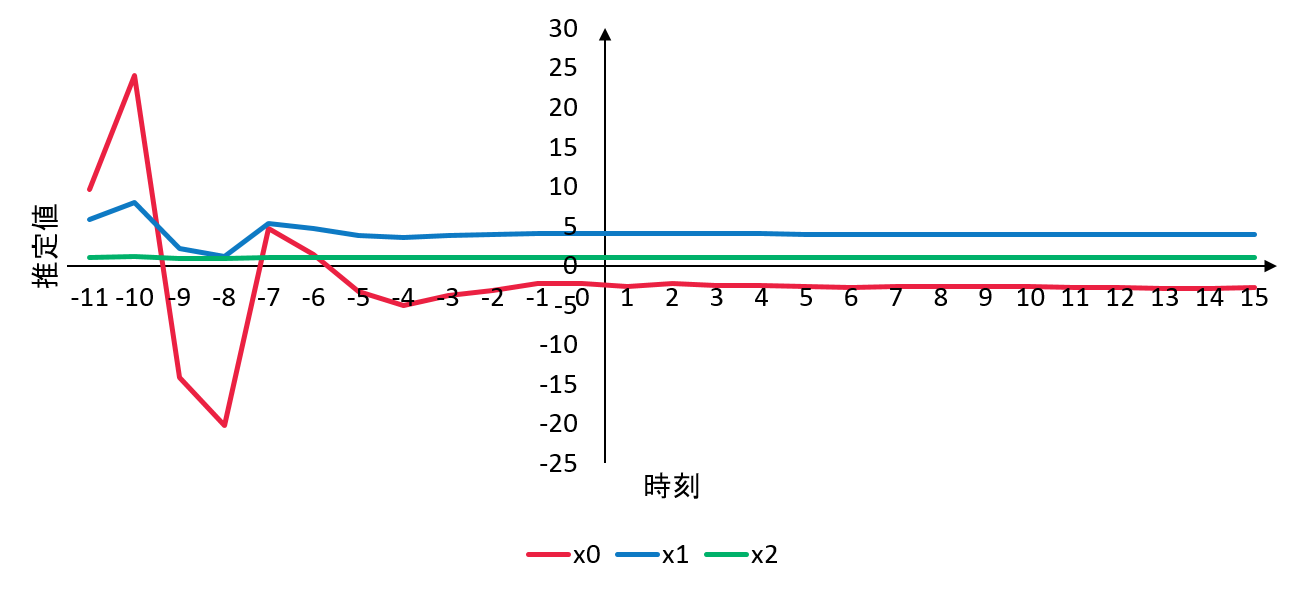
\includegraphics[width=16cm]{Sequen.png}
  \caption{逐次型最小二乗法による推定値の時系列グラフ(-11$\le a \le $15)}
 \label{graph}
\end{figure}

リスト5より,時刻$a$が15のとき推定値は\(x_{0}=-2.773, x_1 = 3.983 x_2 = 0.9999\) となっており,正しく推定できていることがわかる.また,図3より,推定値が収束していることがわかる.
%-----------------------------
%4章
%-----------------------------
\newpage
\section{逐次型最小二乗法における初期推定誤差共分散に対する推定精度}
逐次型最小二乗法では,任意の時刻の1つ前の時刻の推定値が必要となるが,最初の時刻では,1つ前に推定値が存在しないため推定することができない.そこで,初期推定値を0とし,初期推定誤差共分散を適当に設定して推定精度の検証を行う.このとき推定誤差は,
\(
\mbox{\boldmath $P$}_{(0)} =
\begin{bmatrix}
{p} & \cdots & 0\\
 \vdots & \ddots & \vdots\\
0 & \cdots & {p} \\ 
\end{bmatrix} 
\)
となるように設定する.\(p=10^{-6}, 10^{-3}, 10^{0}, 10^{3}, 10^{6}\)であるときの,逐次型最小二乗法による推定値の時系列グラフを図4-8に示す.

\begin{figure}[!h]
  \centering
  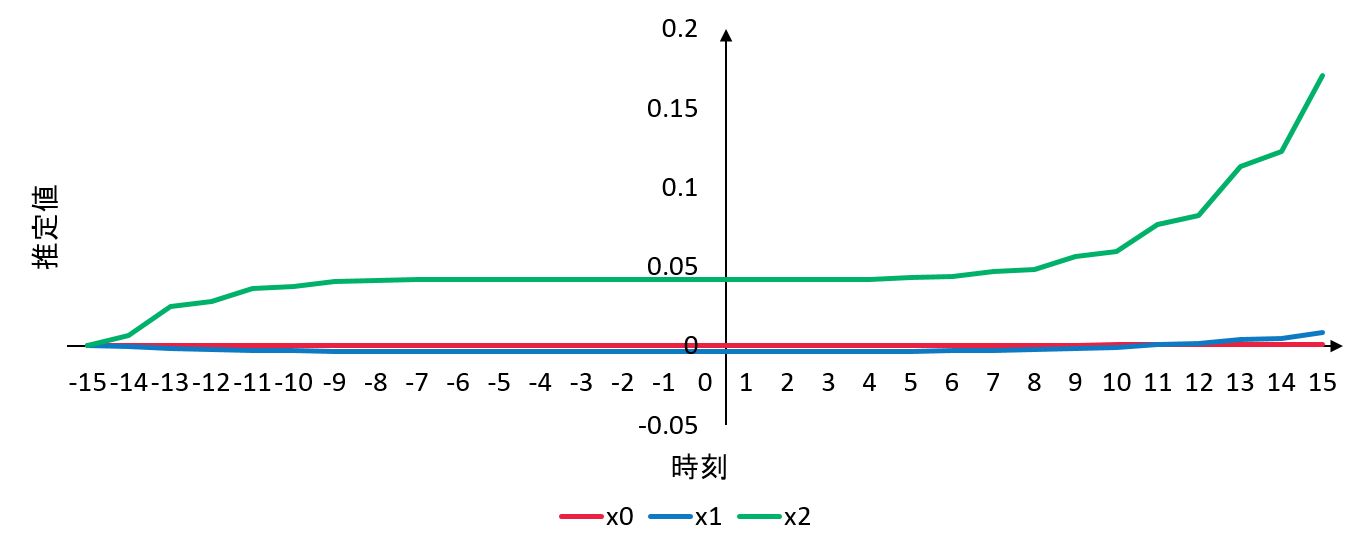
\includegraphics[width=16cm]{Seq-6.png}
  \caption{逐次型最小二乗法による推定値の時系列グラフ\( (p=10^{-6}) \)}
 \label{graph}

  \centering
  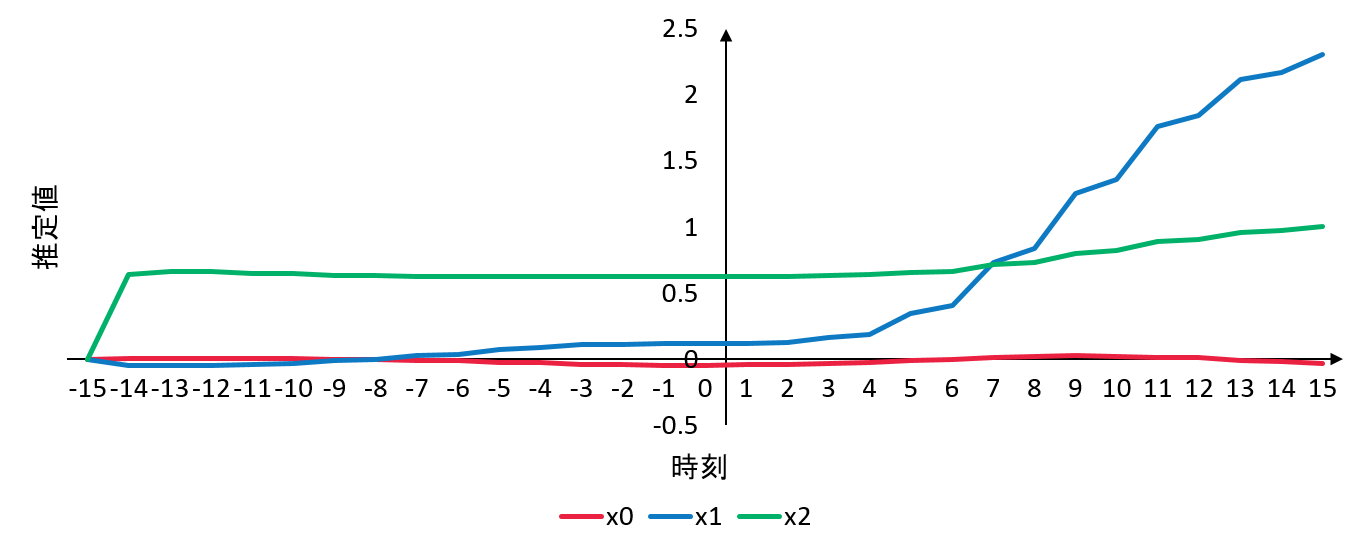
\includegraphics[width=16cm]{Seq-3.png}
  \caption{逐次型最小二乗法による推定値の時系列グラフ\( (p=10^{-3}) \)}
 \label{graph}
\end{figure}
\begin{figure}[!h]
  \centering
  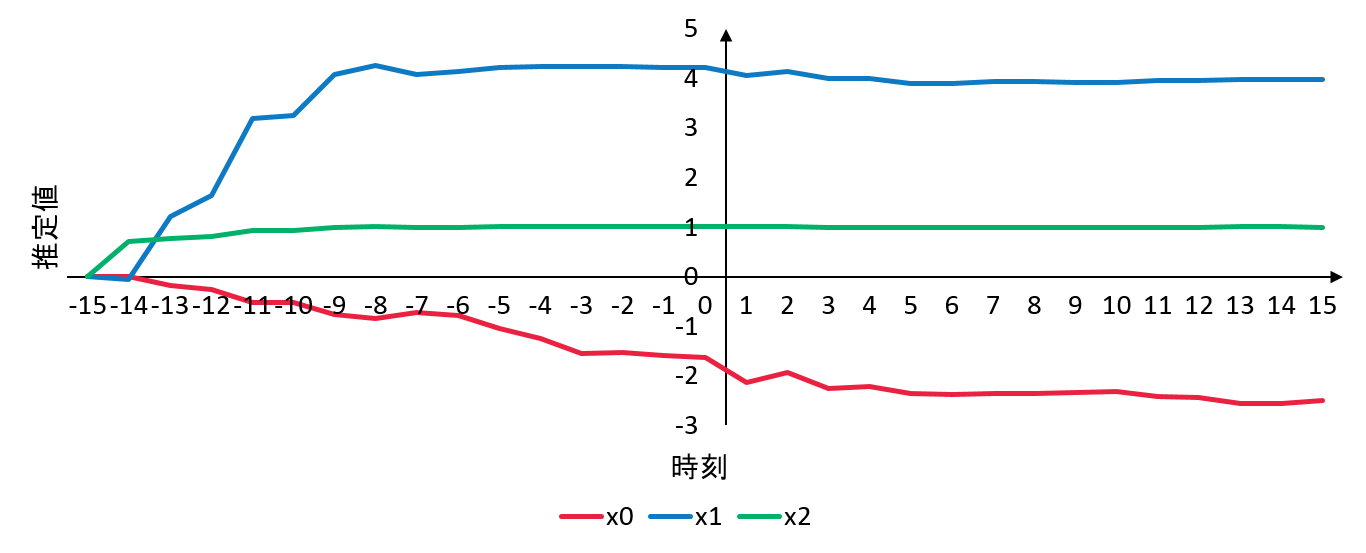
\includegraphics[width=16cm]{Seq0.png}
  \caption{逐次型最小二乗法による推定値の時系列グラフ\( (p=10^{0}) \)}
 \label{graph}

  \centering
  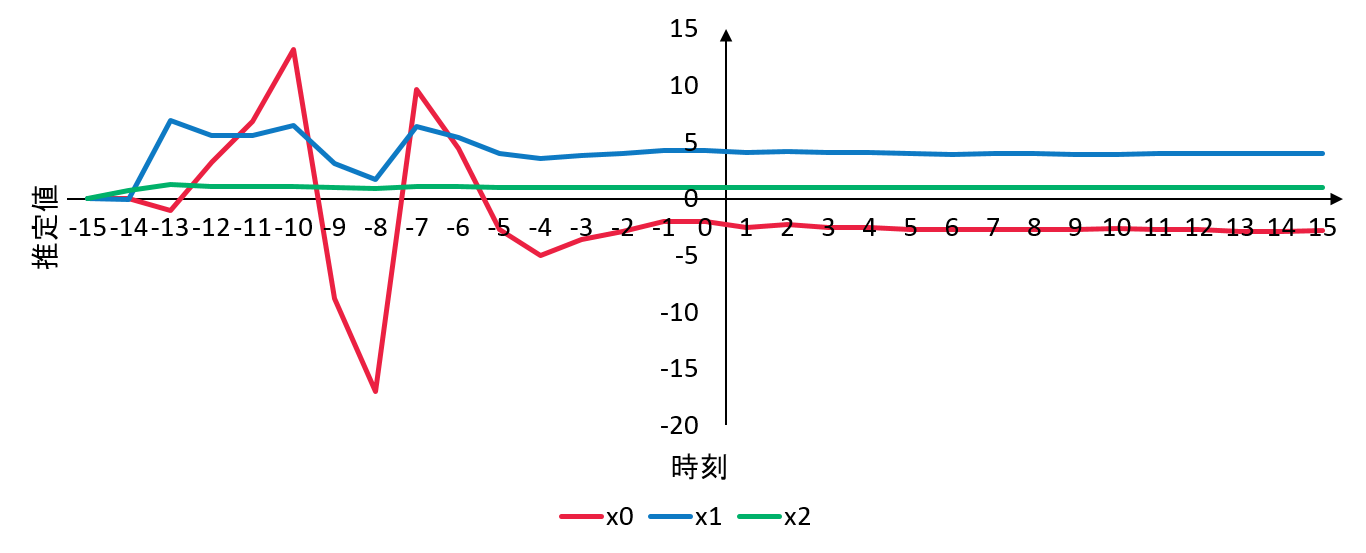
\includegraphics[width=16cm]{Seq3.png}
  \caption{逐次型最小二乗法による推定値の時系列グラフ\( (p=10^{3}) \)}
 \label{graph}

  \centering
  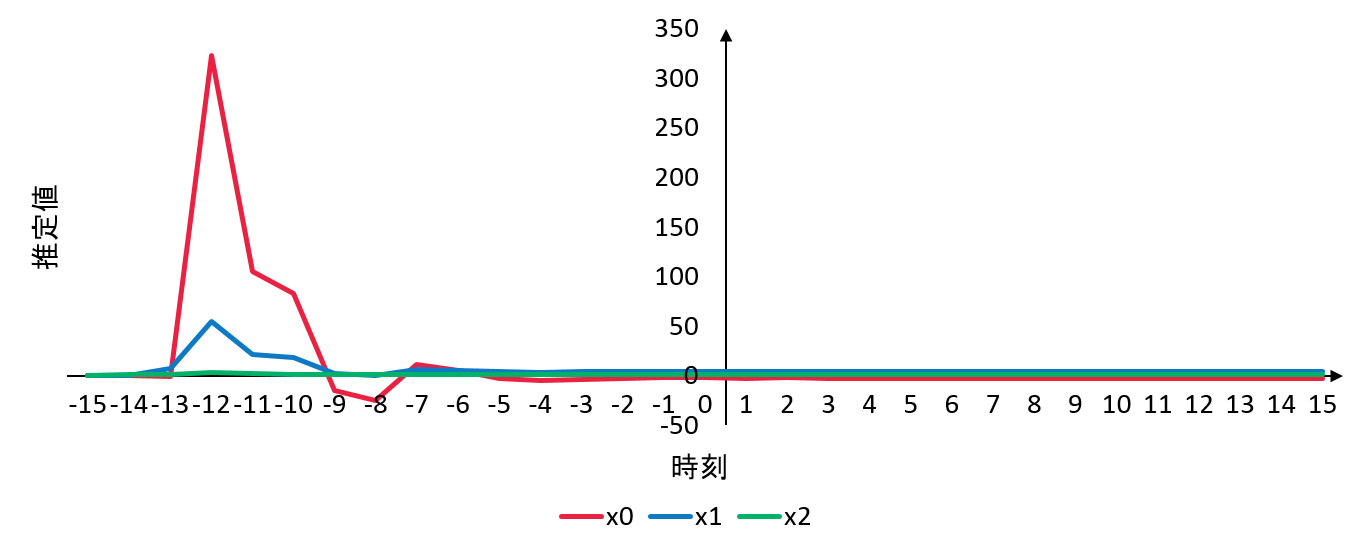
\includegraphics[width=16cm]{Seq6.png}
  \caption{逐次型最小二乗法による推定値の時系列グラフ\( (p=10^{6}) \)}
 \label{graph}
\end{figure}

図4-8より,初期推定誤差共分散の値が小さくなればなるほど推定する時間が長くなるため,収束することができないので推定できないことがわかる.
一方,初期推定誤差共分散の値が大きくなれば大きくなるほど,最初の時刻での誤差が非常に大きくなるが,その後収束するので推定が可能であることがわかる.
これより,初期推定誤差共分散を非常に大きくすることで推定誤差が小さくなることがわかる.
これは,推定誤差共分散が小さいということはその値が真値に近いことを示しているためあまり補正されないが,推定誤差共分散が大きいと真値から離れていることを示すので大きく補正がされることが原因であると考えられる.
\end{document}